Описание выбранных методов, моделей, алгоритмов решения задач.
Во-первых описывается общая трехкомпонентная архитектура программы.
Во-вторых с аппаратной точки зрения описываются платформы на которых будут исполнятся компоненты программы.
В-третьих описывается архитектура каждого компонента и их модулей.
В-четвертых описывается модель взаимодействия между модулями внутри каждого компонента.
В-пятых описывается модель взаимодействия между тремя компонентами программы.

\subsection{ Архитектура программы }
Программа имеет трехкомпонентную архитектуру. Первым компонентом является прошивка, устанавливаемая на РВ-90. Второй компонент представляет собой одно-страничное веб-приложение, которое будет храниться во флеш-памяти вместе с прошивкой, передаваться на устройство пользователя при подключении и запускаться в браузере. Третий компонент - это Android-приложение, которое может быть установлено на устройстве пользователя через Google Play[12]. Каждый компонент создается с использованием своего стека технологий. Таким образом, программа состоит из трех отдельных компонентов, которые должны быть разработаны отдельно и должны будут взаимодействовать друг с другом. 
 
Конструкция аппаратной базы для РВ-90 является фиксированной и должна учитываться при проектировании архитектуры программы

\textbf{Три платформы}
\begin{my_itemize}
\item РВ-90
\item Браузер
\item Android
\end{my_itemize}


\begin{figure}[h!]
    \centering
    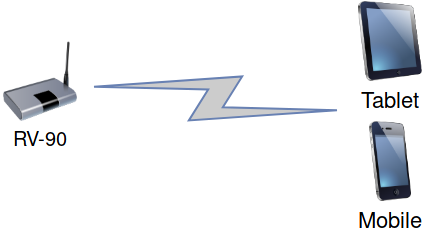
\includegraphics[width=0.9\textwidth]{three_platforms.png}
    \caption{Диаграмма взаимодействия между реле и клиентом.}
\end{figure}



%===========================================================================



\newpage
\subsection{ Платформа РВ-90 }
Аппаратная база представлена в виде устройства РВ-90. Нет смысла рассматривать абсолютно все физические характеристики устройства. Далее будут рассмотренны те из них, которые влияют на реализацию программы. В основе устройства находится модуль RAK473. К GPIO вводам которого подключены: 3 пина для программирования (SWDIO, SWCLK, RST), 2 пина для взаимодействия через UART (RX, TX), питание 5 вольт, земля, шина I2C. К шине I2C подключены часы реального времени DS1307 и I2C расширитель портов PCA9555. К GPIO выводам расширителя подключены 4 светодиода, 3 push-down кнопки, 2 реле RT424005.
Выбор компонентов влияет на архитектуру программы. В данной секции в больших деталях рассмотренны некоторые компоненты РВ-90 и их аналоги с целью понимания специфики каждого компонента. 

\subsubsection{ Разбор кнопок на корпусе РВ-90 }
На корпусе имеются 3 кнопки, 2 из них для ручного переключения состояния каждого из двух реле, и одна для жесткой перезагрузки системы.
Кнопки не используют пин прерывания имеющийся у I2C расширителя портов RCA9555 для оповещения об изменении своего состояния. Программа должна периодически опрашивать текущее напряжение на кнопках, чтобы заметить нажатие. По умолчанию линии кнопок притянуты вверх, поэтому напряжение уровня земли соответствует нажатию. Программа должна применять фильтр к данным о состоянии кнопок, чтобы исключить ложные срабатывания, а также и двойные/тройные срабатывания из-за дребежзания контактов. 

\subsubsection{ Разбор I2C расширителя портов PCA9555 } 
Выбор I2C расширителя портов PCA9555 обоснован его низкой ценой и расширением на 16 GPIO портов, которых более чем хватает для контроля аналоговой периферии, и возможностью задать I2C адрес для расширителя на этапе производства устройства, чтобы избежать конфликта адресов на шине. В качестве аналога существует более дешевый PCA9554 предоставляющий расширение на 8 GPIO портов и имеющий жестко зафиксированный адрес на шине. 

\subsubsection{ Разбор часов реального времени DS1374 }
Выбор часов реального времени DS1374 имеет недостаток в виде высокой цены и много достоинств. 
Для взимодействия с микроконтроллером данные часы используют протокол I2C, вместе с другой периферией их можно подключить к общей шине I2C, что очень важно в условиях ограниченного колличества GPIO пинов  микроконтроллера.
Данные часы отсчитывают время в формате Unix-time. Формат Unix-time удобен для хранения, сравнения и передачи. Поскольку подразумевается что пользователь может создавать много событий включения/выключения требующих хранения времени, а память в системе ограничена, то важно иметь компактный формат для хранения времени. При взаимодействии с пользователем и при работе программы временные значения будут часто передаваться между различными програмными модулями, важно что формат Unix-time очень прост в представлении и следовательно удобен для передачи. При принятии решений система должна уметь возможность сравнивать и считать разницу между двумя временными значениями, время в формате Unix-time можно удобно и быстро сравнивать между собой (простое сравнение 32-битных целых чисел). Недостатком формата Unix-time в том что он не может отразить дополнительные високосные секунды [\url{https://stackoverflow.com/a/50910322/1073672}], а также в том что он может отображать только даты в промежутке с 1901 по 2038 год. Также в январе 2038 года данный формат будет подвержен ошибке из-за переполнения 32-битного целого числа. Программа для управления РВ-90 работает лишь с текущим годом, плюс-минус 10 лет, поэтому в данной работе ошибка переполенния никак не обрабатывается. Что касается дополнительных високосных секунд, то с 1970 по 2007 их было 23 [\url{http://pubs.opengroup.org/onlinepubs/9699919799/xrat/V4_xbd_chap04.html#tag_21_04_15}], поэтому за период эксплуатации устройства, состовляющий ориентировачно 2 года ожидается что их влияние будет несущественно. Тем не менее программа предоставляет пользователю возможность синхронизировать время в РВ-90 с другим устройством с целью устранения ошибки в отсчете времени на РВ-90. Часы DS1374 также имеют возможность генерировать программируемое прерывание.
Прерывания в определенный момент времени можно использовать для максимально точного контроля реле. Однако, в такой точности нет необходимости поскольку текущее время с точностью до секунды можно отсчитывать центральным процессором. Поэтому часы используются для борьбы с небольшой плавающей ошибкой, для этого программа синхронизируется с часами один раз в час. Также часы используются для бесперебойного отсчета времени когда устройство РВ-90 не подключено к электропитанию, для этого часы имеют отдельное питание от батарейки. Надо учитывать что часы используют 32-битное знаковое целое число для счетчика и подвержены ошибке переполнения счетчика в 2038 году. В данной работе эта ошибка не обрабатывается.  
В качестве аналога к часам DS1374 имеются часы DS1672, которые практически идентичны за исключением возможности генерации прерывания. 
Программа не имеет функционала для работы с часами использующими представление времени в формате BCD (Binary Coded Decimal). Часы в формате BCD удобны для вывода времени, кроме того они корректно отсчитывают текущую дату и время, принимая в расчет високосные года. В частности дополнительный день и секунды в високосный года, а также количество дней в каждом месяце в зависимости от текущего года. 
Пример часов работающих в формате BCD - DS1307, отличаются низкой ценой.


\subsubsection{ Разбор модуля РАК473 }
Производства компании Rak-Wireless [\url{http://docs.rakwireless.com/en/WIFI/RAK473/Hardware%20Specification/RAK473%C2%A0UART%C2%A0WiFi%C2%A0Module%C2%A0Specification%20V1.5.pdf}]. 
Существует аналогичный модуль компании FN-link F11AMIM13\_B1. RAK473 включает в себя микроконтроллер RTL8711AM от Realtek, флеш-память GD25Q16C размером в 2MB от GigaDevice подключаемую к микроконтроллеру через SPI интерфейс, Wi-Fi антенну, регуляторы и предохранители для GPIO пинов чипа. Блок схема модуля представленна на рисунке.

\begin{figure}[h!]
    \centering
    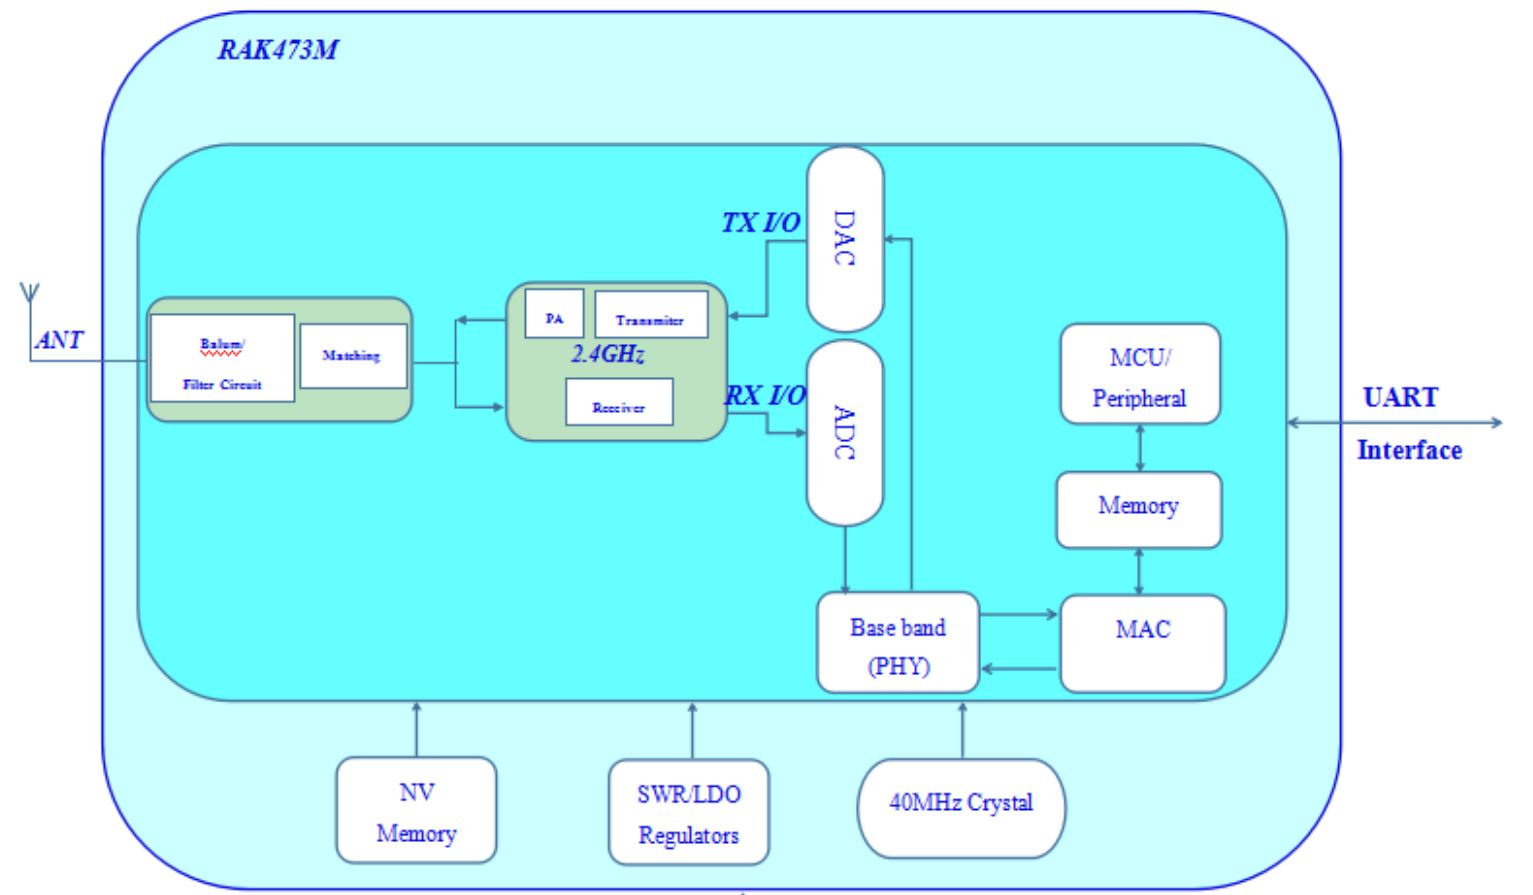
\includegraphics[width=0.9\textwidth]{rak473_block_diagram.png}
    \caption{Блок схема модуля на рисунке.}
\end{figure}

У модуля имеются 19 GPIO. 
Выводы GPIOB0 и GPIOB1 используются для UART.
Выводы GPIOB2, GPIOB3 используются для подключения шины I2C.
Выводы GPIOE4, GPIOE3 используются для программирования.
Схема GPIO выводов модуля представленна на рисунке.

\begin{figure}[h!]
    \centering
    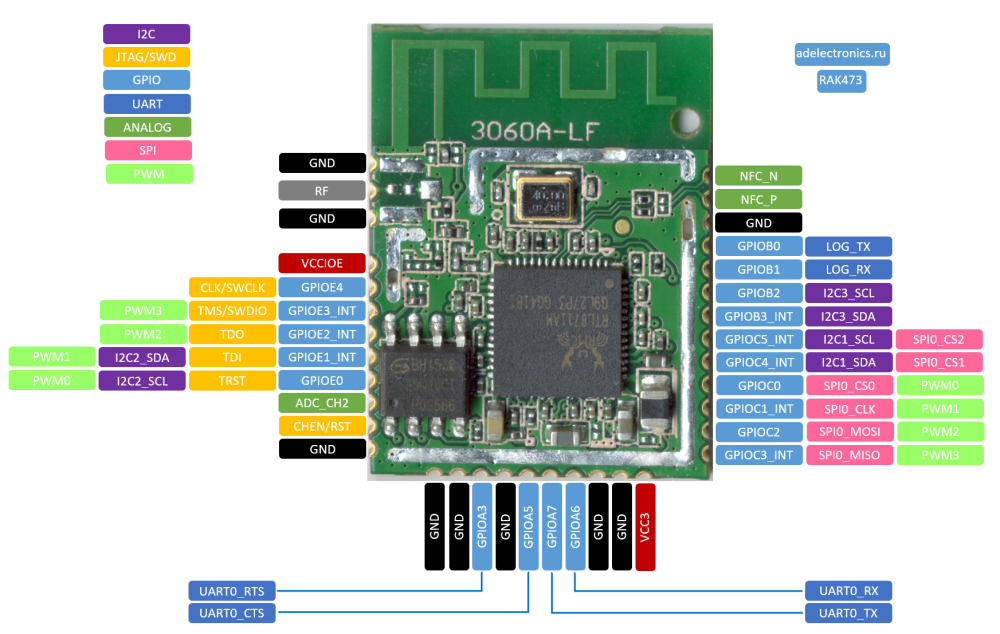
\includegraphics[width=0.9\textwidth]{rak473_pinout.png}
    \caption{Схема GPIO выводов модуля RAK473.}
\end{figure}

\subsubsection{ Разбор микроконтроллера RTL8711AM }
В основе модуля RAK473 находится микроконтроллер производства компании Realtek[7]. Это одно-кристальный микропроцессор нацеленный для изделий Internet of Things. Он сочетает в себе ARM ядро на базе Cortex-M3, WLAN MAC и NFC в одном чипе. Тактовая частота процессора 166 MHz. 

Процессор имеет 1MB встроенной ROM памяти, 2.5 MB RAM памяти и SPI интерфейс для подключения Flash памяти.  В памяти ROM размещается заводской бутлоадер и некоторые функции для стандартной библиотеки. Данная память находится по адресам с 0х00000000 по 0х000FFFFF. Ей невозможно воспользоваться для разработки, т.к. ее невозможно перепрошить. Память RAM состоит из блока SRAM и блока SDRAM. SRAM (Static Random Access Memory) это статичная память, доступ к ячейкам данного типа памяти осуществляется быстрее чем к ячейкам памяти SDRAM (Synchronous Dynamic Random Access Memory), к тому же ее не надо периодически обновлять чтобы поддерживать правильные значения битов памяти. Однако она дороже т.к. требует большего колличества трансисторов на один бит памяти. Поэтому в данном микроконтроллере память SRAM имеет всего лишь 448KB. SRAM расположена по адресам с 0х10000000 по 0х1006FFFF. Память SDRAM имеет 2 МB памяти. Доступ осуществляется по адресам с 0х30000000 по 0х301FFFFF.

При записке микроконтроллер начинает с исполнения заводской программы, то есть загрузчика (bootloader) находящегося в ROM памяти. Загрузчик инициализирует некоторые внутренние значения и переходит к считываению данных из подключенной флеш-памяти. Ожидается что память подключена по протоколу SPI к определенным пинам микроконтроллера. 
Ниже предствалено разбиение флеш-памяти с которым ожидает работать загрузчик. Изображение ниже не является картой RAM памяти. 

\begin{figure}[h!]
    \centering
    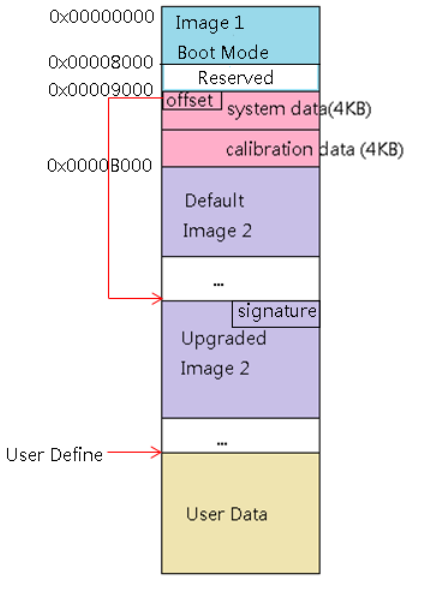
\includegraphics[width=0.4\textwidth]{rtl8711am_flash_layout.png}
    \caption{Разбиение флеш-памяти с которым ожидает работать загрузчик.}
\end{figure}

На схеме также показан "Upgraded Image 2", который используется для технологии обновления прошивки OTA (Over The Air). Данная программа не предусматривает возможности обновления прошивки по каналу Wi-Fi, поэтому область выделенная для "Upgraded Image 2" может быть использованна для любых других нужд разработчика. В частности для хранения пользовательской информации.


Загрузчик поддерживает работу с форматом Binary Image File (.bin). Для того чтобы получить прошивку (файл типа .bin) которая будет правильно обработана загрузчиком следует использовать оффициальный SDK (Software Development Kit) от компании Realtek. Загрузчик читает данные из флеш-памяти и в соответствии с директивами формата ELF копирует данные в разные области RAM памяти. После этого загрузчик очищает свой стек и передает управление пользовательскому коду. Таким образом RTL8711AM не использует технологию XiP (Execute in Place), хотя она и является довольно распространенным решением.

\subsubsection{ Разбор ядра ARM Cortex-M3 }
В основе микроконтроллера RTL8711AM находится ядро ARM Cortex-M3. Это семейство процессоров, призванное занять новую для ARM нишу встраиваемых решений. В семействе присутствуют три значимых ядра[The definitive guide to arm cortex m3 by Joseph Yiu].

\begin{my_enumerate}
\item Cortex-M0 с архитектурой ARMv6-M;
\item Cortex-M3 (опционально Memory Protection Unit) с архитектурой ARMv7-M;
\item Cortex-M4 (опционально Floating Point Unit) с архитектурой ARMv7E-M;
\end{my_enumerate}

Диаграмма ниже отображает какие подсистемы процессора реализуются по спецификации ARM, а какие по инициативе конкретных компаний, таких как Realtek.

\begin{figure}[h!]
    \centering
    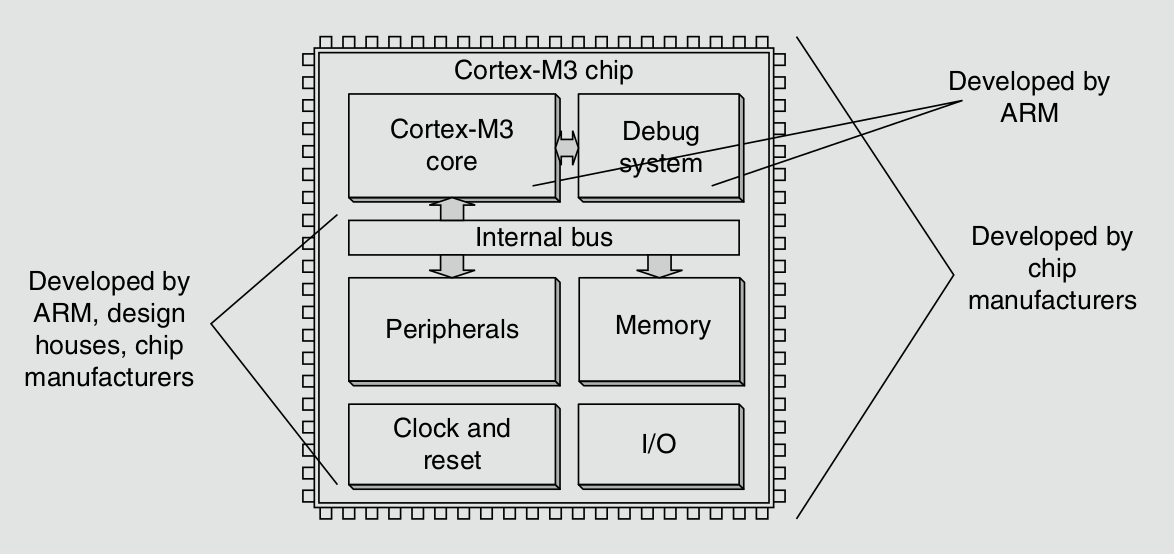
\includegraphics[width=0.6\textwidth]{arm_vs_custom_modules.png}
    \caption{Разбиение реализации подсистем процессора.}
\end{figure}


Процессор использует Гарвардскую архитектуру, имеется отдельная шина инструкций и шина данных. Однако шины инструкции и данных используют единое пространство памяти. Поэтому общая память системы делится между данными и инструкциями. Процессор Cortex-M3 включает в себя ряд фиксированных внутренних компонентов отладки которые разрабатываются компанией ARM. Эти компоненты обеспечивают поддержку операций отладки и функции, такие как точки останова (breakpoints) и точки наблюдения (watchpoints).

\begin{figure}[h!]
    \centering
    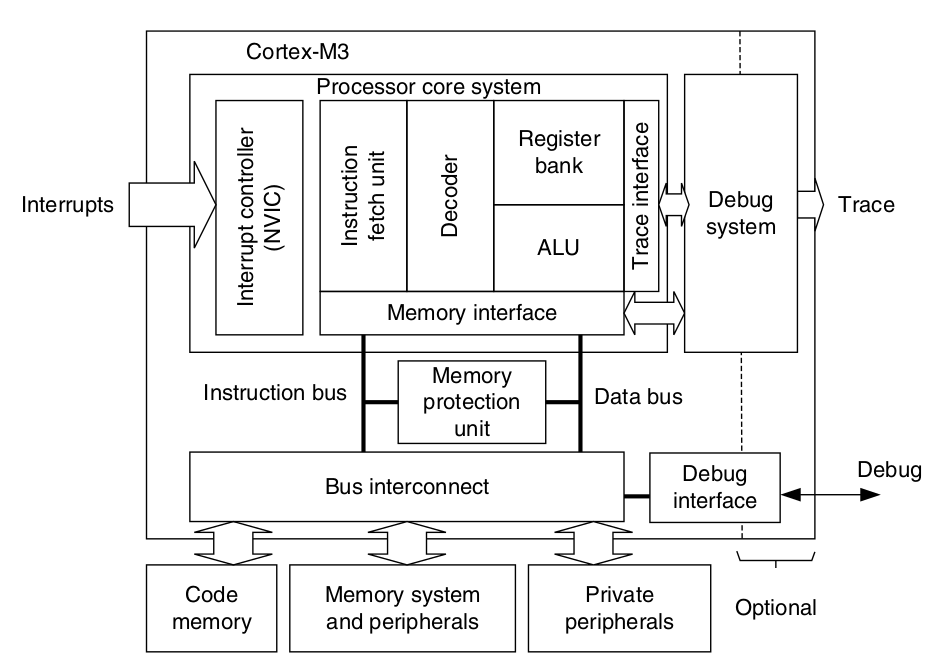
\includegraphics[width=0.6\textwidth]{cortex_m3_subsystems_overview.png}
    \caption{Подсистемы процессора Cortex-M3.}
\end{figure}


Функционал Trace отключен. Подсистема MPU (Memory Protection Unit) не поддерживается.
Процессор имеет два режима работы: Превелигированный и пользовательский режим. В данной работе используется только превелигированный режим. Cortex-M3 предоставляет стандартизированную схему разбиения адресов для разработчиков микроконтроллеров. Это важно для функционирования программы поскольку определяет способ для взаимодействия между программой на C и периферией процессора. В данном случае доступ к периферии производится обращением к определенным ячейкам памяти. Производители могут модифицировать схему разделов памяти. Как описано в разделе о границах RAM памяти Realtek немного модифицировал рабиения памяти. ROM память находится по адресам с 0х00000000 по 0х000FFFFF. SRAM расположена по адресам с 0х10000000 по 0х1006FFFF. Доступ к памяти SDRAM осуществляется по адресам с 0х30000000 по 0х301FFFFF.
 
\begin{figure}[h!]
    \centering
    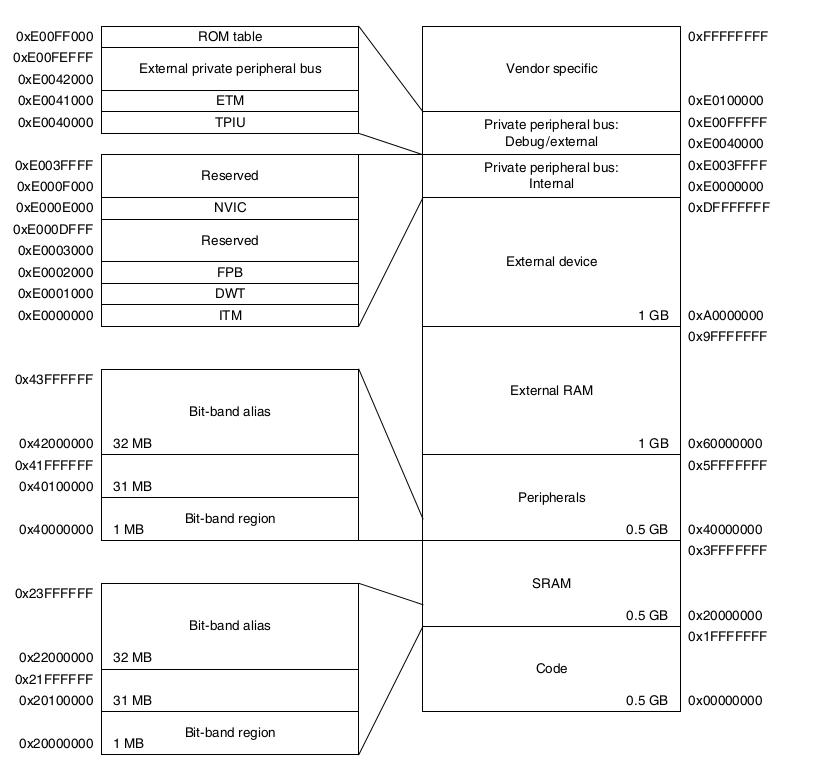
\includegraphics[width=0.9\textwidth]{predefined_memory_map.png}
    \caption{Разбиение памяти для микроконтроллера Cortex-M3.}
\end{figure}


Поддержка аппаратных прерываний осуществляется с помощью NVIC (Nested Vectored Interrupt Controller). Важными особенностями NVIC для функционирования программы являлось то что он поддерживает вектор прерываний (vectored interrupt support), вложенные прерывания на аппратном уровне (nested interrupt support), програмно устанавливаемые приоритеты для прерываний (dynamic priority changes support), маскировку прерываний (interrupt masking).


Процессор взаимодействует с периферией через несколько шин. Ниже представлена блок-схема подключения периферии включая шину для отладки внутри процессора.

\begin{figure}[h!]
    \centering
    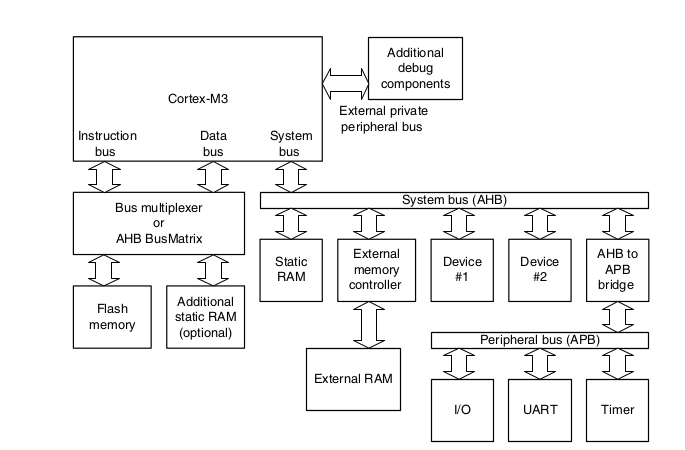
\includegraphics[width=0.8\textwidth]{cortex_m3_peripherals_block_diagram.png}
    \caption{Блок-схема подключения периферии к шинам внутри процессора.}
\end{figure}


Процессор Cortex-M3 включает в себя функции отладки. Поддерживает JTAG или SW (Serial-Wire) интерфейс для внешнего отладчика. Технология реализующая подсистему отладки процессора - CoreSight. С ее помощю можно получить доступ к состоянию регистров процессора и содержимому ячеек памяти. Есть встроенная поддержка шести точек останова (breakpoints) и четырех точек наблюдения (watchpoints). [CoreSight Technology System Design Guide]

В Cortex-M3, доступ к функционалу для отладки расположенному на процессоре осуществляется через интерфейс шины DAP (Debug Access Port). DAP управляется другим компонентом известным как DP (Debug Port) который преобразует команды JTAG или SW (Serial-Wire) поступающие из внешнего отладчика в команду DAP и направляет ее на шину. Ниже приведены схема подключения отладчика к процессору, а также  схема взаимодействия компонентов отладки Cortex-M3. 


\begin{figure}[h!]
    \centering
    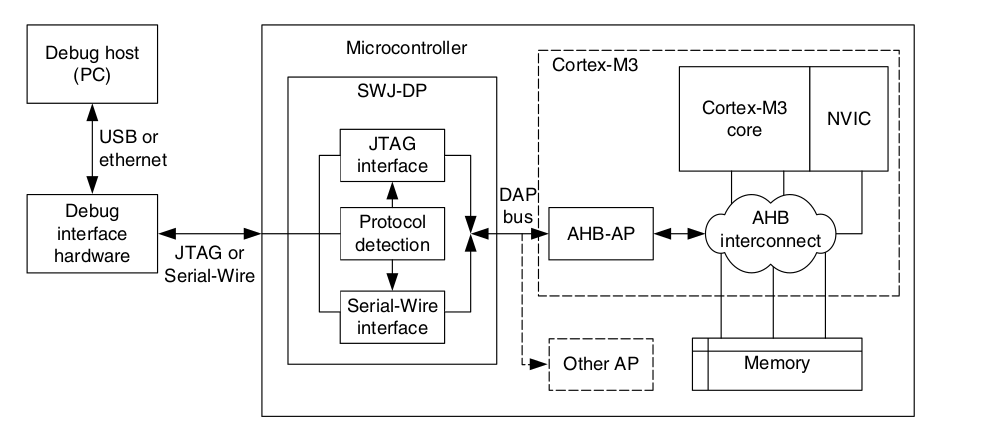
\includegraphics[width=0.9\textwidth]{cortex_m3_debug_connection.png}
    \caption{Схема подключения отладчика к процессору Cortex-M3.}
\end{figure}


\begin{figure}[h!]
    \centering
    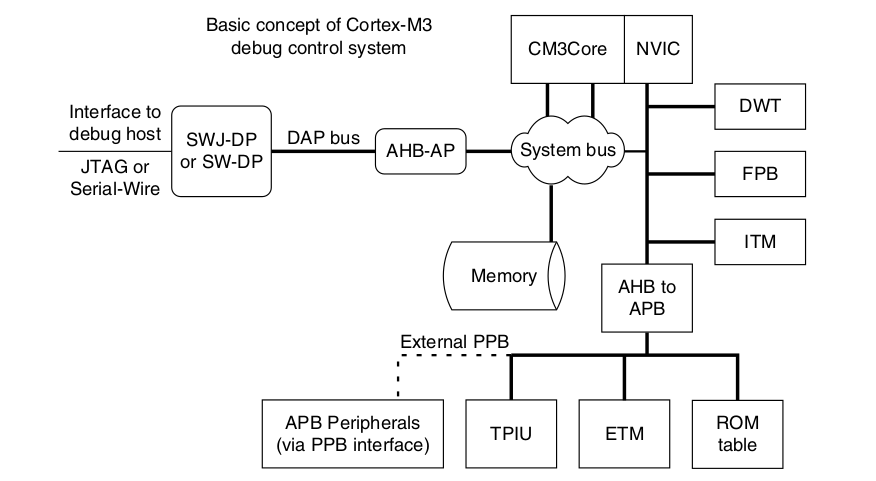
\includegraphics[width=0.9\textwidth]{cortex_m3_inside_debug_subsystem.png}
    \caption{Схема взаимодействия компонентов отладки Cortex-M3.}
\end{figure}

.


\newpage

\subsection{Платформа Браузер}
На самом деле не следует рассматривать конкретный браузер как платформу для разработки. Следует рассматривать набор спецификаций которые суммарно определяют веб-платформу. Браузер лишь реализует данные спецификации и предоставляет разработчику доступ к конкретной имплементации веб-платформы.

\subsubsection{ Организации выпускающие спецификации веб-платформы}
Стандарты публикуемые организацией W3C определяют основные компоненты веб-платформы. Границы веб-платформы продолжают развиваться. Краеугольным камнем веб-платформы является HTML5, однако функционал используемый в данной работе зависит от многих других спецификаций, которые создают W3C и другие организации. В частности CSS, SVG, WOFF, ECMAScript и различные браузерные API.

В разработке спецификаций которые опеределяют веб-платформу участвуют несколько организаций. Ниже перечисленны ключевые организации публикующие стандарты которые определяют веб-платформу.

\begin{my_enumerate}
\item Рекомендации, опубликованные консорциумом World Wide Web Consortium (W3C) [2], такие как HTML / XHTML, каскадные таблицы стилей (CSS), объектная модель документа (DOM), форматы изображений, такие как портативная сетевая графика (PNG) и масштабируемая векторная графика (SVG), а также специальные технологии, такие как WOFF.
\item Стандарты, опубликованные Ecma International (ранее ECMA) [4], такие как JavaScript (также известный как "стандартный ECMAScript")[3]
\item Стандарты, опубликованные международной организацией по стандартизации (ISO) [5], такие как JPEG.
\end{my_enumerate}


\subsubsection{ Спецификации определяющие веб-платформу}
Набор спецификаций определяющий веб-платформу позволяет разработчику абстрагироваться от конкретного браузера. Это существенно облегчает разработку веб-приложения которое должно работать в различных браузерах.

Когда веб-сайт или веб-приложение описываются как соответствующие стандартам веб-платформы или просто веб-стандартам, это означает, что сайт или приложение имеют допустимые стандартом HTML, CSS и JavaScript. HTML отвечает требованиям доступности для людей с нарушением зрения (дальнозоркостью или дальтонизмом) или движений, благодаря размещению специальных пометок и дополнительной информации на странице, а также другим семантическим рекомендациям. Полное соответствие стандарту охватывает также корректные параметры для кодирования символов, корректные метаданные, корректно сформированный XML, корректное встраивание скриптов и правильную настройку сервера.

Компонент программы который предназначен для исполнения в браузере, то есть для запуска на веб-платформе, требует для успешной работы чтобы браузер поддерживал следующие основополагающие спецификации описывающие веб-платформу.

\begin{my_enumerate}
\item Рекомендации для языков разметки, таких как язык разметки HTML (HyperText Markup Language) и масштабируемая векторная графика (Scalable Vector Graphics) из W3C.
\item Рекомендации для таблиц стилей, особенно каскадных таблиц стилей (Cascading Style Sheets), от W3C.
\item Стандарты для ECMAScript, чаще JavaScript, от Ecma International.
\item Рекомендации для объектных моделей документов (Document Object Model) от W3C.
\item Правильно сформированные имена и адреса для страницы и всех других ресурсов, на которые в ней есть ссылки (Uniform Resource Idenfirier), на основе RFC 2396, из IETF.[12]
\item Правильное использование HTTP и MIME типов для скачивания веб-страницы, ее интерпретации и запроса других ресурсов, упомянутых в ней, на основе RFC 2616, из IETF.[13]
\item Веб-доступность обычно основана на руководящих принципах доступности веб-контента[14], опубликованных инициативой W3C по веб-доступности.
\end{my_enumerate}

\subsubsection{ Реализация веб-платформы в различных браузерах}
При создании компонента программы для веб-платформы важно помнить что в итоге компонент должен будет запускаться на конкетной версии конкретного браузера на конкретном пользовательском устройстве (операционной системе).
Разработка компонента для браузера не тривиальна, в силу того что существует несколько популярных браузеров, у многих есть мобильные версии, у одного браузера есть несколько популярных устаревших версий браузера, и наконец для каждой операционной системы существует своя версия браузера. Каждая из этих мобильных или десктопных версий является своей обособленной реализацией веб-платформы. Каждая из этих мобильных или десктопных версий имеет свои уникальные ошибки и недосмотры в реализации стандартов описывающих веб-платфрому. Веб-разработчик сталкивается с проблемами дырявых абстракций (leaky abstractions)[https://www.joelonsoftware.com/2002/11/11/the-law-of-leaky-abstractions/] в том как браузеры реализуют стандарты описывающие веб-платформу.


\subsubsection{ Поддерживаемые браузеры}
Из-за большого количества различных реализаций веб-платформы невозможно вести разработку нацеленную на правильную работу во всех браузерах. Необходимо выделить реальное подмножество на которое будет нацелена разрабокта из множества всех комбинаций версий, типов браузеров и версий, типов операционных систем.

При разработке компонента для запуска в браузере следует учитывать что после его интерграции в программу для управления и мониторинга РВ-90 у разработчика не будет возможности что-либо изменить в данном компоненте. В дилу данного факта следует уделить уделить особое внимание правильному пониманию и использованию стандартов описывающих веб-платформу, а также следует стремиться максимально расширить множество поддерживаемых браузеров, чтобы охватить как можно больше наиболее распространенных версий.

Следует определить каким именно браузерам стоит уделить внимание при разработке. 
Для данной программы было решено ограничеться поддержкой браузеров которые имеют более 0.05\% рынка пользователей в России, при этом исключив из этого списка браузеры Internet Explorer версии 9 и раньше, а также браузер Opera mini. Для определения конкретных версий и названий браузеров, которые должны стать ключевыми при реализации были использованы проекты "Can i use" и "Browserlist".

Также не представлялось возможным осуществить поддержку каждой из всех 30 распространенных версий Gogole Chome и Firefox поэтому для тестирования были выбраны самые новые и самые старые из популярных версий каждого браузера.
Ниже приведен итоговый список поддерживаемых браузеров для программы управления и контроля РВ-90.

\textbf{Мобильные браузеры}
\begin{my_itemize}
\item Chrome for Android 73
\item Firefox for Android 66
\item UC Browser for Android 11.8
\item Android Browser 4.4
\item Android Browser 4
\item IE Mobile 11
\item iOS Safari 12
\item iOS Safari 8
\item Samsung Internet 9.2
\item Samsung Internet 7
\end{my_itemize}

\textbf{Десктопные браузеры}
\begin{my_itemize}
\item Chrome 74
\item Chrome 52
\item Firefox 66
\item Firefox 48
\item Edge 18
\item IE 10
\item Opera 58
\item Opera 39
\item Safari 12
\item Safari 9
\end{my_itemize}

Приведенные выше браузеры являются поддерживаемыми платформами для работы одно-страничного веб-приложения являющимся одним из трех компонентов программы для управления РВ-90.


\newpage
\subsection{Платформа Android}







%===========================================================================



\newpage
\subsection{Архитектура прошивки для РВ-90}
% what is it
% what it does
Прошивкой является файл типа .bin который прошивается во флеш-память находящуюся на модуле.

\subsubsection{ Прошивка для РВ-90 }
Файл прошивки получается на последнем этапе компиляции, посредством обработки EFL (Executable and Linkable Format, Extensible Linking Format) файла программы. 
Файл Bin - это чистый двоичный файл без исправлений памяти или перемещений, он требует загрузки по определенному адресу памяти.
Файлы ELF - это более сложный формат, состоящий из секций не все из которых предназначенны для загрузки в RAM память. Формат включает в себя таблиц для поиска символов и таблицы перемещений. Он предназначается для загрузки операционной системой по произвольному адресу памяти, адреса переменных в этом случае вычисляются во время выполнения используя таблицу GOT (Global Offset Table). 
Ниже представлена шема сборки прошивки с помощью оффициального SDK от Realtek и GNU GCC ARM Toolchain.
 
\begin{figure}[h!]
    \centering
    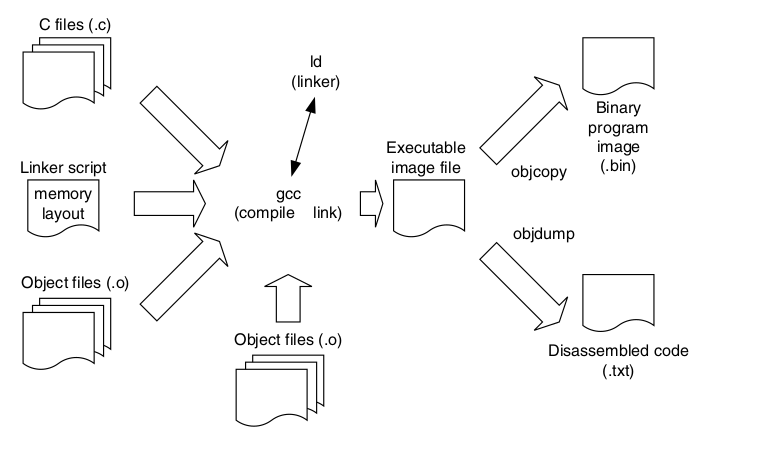
\includegraphics[width=0.7\textwidth]{compilation_steps_firmware.png}
    \caption{Этапы сборки прошивки РВ-90.}
\end{figure}
 

Что должна делать прошивка.
Безопасность и надежность являются первостепенными задачами. На основе анализа соответствующей работы был разработан ряд руководящих принципов и решений. Во-первых, сеть Wi-Fi должна быть размещена самим РВ-90 (рис. 3). Это поможет снизить риск безопасности, связанный с распространением информации через Интернет. Во-вторых, прошивка будет написана на языке программирования Rust. Это ограничит количество ошибок связанных с переполнением буфера, стека и ряда других типичных для приложений написанных на языке C. Использование Rust также должно упростить тестирование, поскольку юнит- тесты являются частью языка, что будет способствовать поддержанию качество кода. Ожидается, что безопасность будет дополнительно повышена путем выбора руководящих принципов MISRA-C, которые могут применяться в контексте языка программирования Rust. 

Использование SoC на основе ARM означает, что Rust может использоваться в качестве языка программирования для выбора прошивки вместо C. необходимо также учитывать тот факт, что флеш-память ограничена 2 МБ. Часть этого пространства должна быть зарезервирована для прошивки, часть для веб-приложения и часть для пользовательских данных. Веб-приложение должно быть как можно меньше, чтобы поместиться во флеш-память вместе с изображениями, шрифтами, библиотеками и другими необходимыми данными. Программа для контроля и мониторинга РВ-90 должна создавать и поддерживать собственную сеть WiFi, чтобы устройство работало даже в зоне без подключения к интернету. Таймер RTC DS1307 имеет разрешение точности до миллисекунды, для того чтобы удовлетворить требованиям для точного времени.

Прошивка устанавливается на РВ-90 в процессе производства.  Прошивка разбивается на несколько модулей. Модули разделены на основе функциональности, которая должна присутствовать в реле времени. Устройство каждого из модулей.

\begin{my_itemize}
\item Модуль управления многозадачностью и аппаратным разделением ресурсов.
\item Модуль для управления выходом реле (включено-выключено).
\item Модуль для работы стека TCP/IP и управления сетью Wi-Fi.
\item Модуль вывода отладочной информации.
\item Модуль управления HTTP сервером.
\item Модуль для анализа и генерации ответа на запросы API.
\item Модуль для анализа и генерации JSON.
\item Модуль для управления коммуникацией по протоколу I2C.
\item Модуль для связи с чипом DS1307 в режиме реального времени.
\item Модуль управления временем системы.
\item Модуль управления файловой системой.
\end{my_itemize}



\subsubsection{ Разбор оффициального SDK от Realtek }
SDK запутанный.



\subsubsection{ Разбор кода предоставляемого компанией ARM}
Вместе с ядром ARM предоставляет стандарт CMSIS  (Cortex Microcontroller Software Interface Standard)
CMSIS предоставляет интерфейс на языке C который реализуется производителями микроконтроллеров, в часности компанией Realtek, для предоставления доступа из языка С к определенным функциям, которые есть на всех процессорах Cortex-M. Для программы контроля и управления РВ-90, важно что данный интерфейс предоставляет функции для доступа к регистрам, NVIC, определения частоты процессора. 




\newpage
\subsection{Архитектура одно-страничного веб-приложения для браузера}
% what is it
% what it does


\subsubsection{ Проектирование архитектуры веб-интерфейса}
Что должен делать каждый из модулей.

Веб-приложение будет написано в Typescript, чтобы свести к минимуму вероятность ошибок во время выполнения.

Пользовательский интерфейс реализован в веб-приложении. Оно предоставляет тот же функционал который можно встретить в других электронных реле времени. Оператор может: создать новый цикл включения/выключения и дать ему имя, назначить цикл определенному дню и установить его на повторение еженедельно или ежемесячно, установить исключения и переопределить циклы в определенные дни, получить обзор того, какие циклы выполняются в какие дни. Интерфейс интуитивно понятен и прост в использовании.

Одно-страничное веб-приложение хранится во флеш-памяти РВ-90 вместе с прошивкой. При подключении оно передается на телефон или планшет пользователя через браузер и в нем же и запускается. Веб-приложение можно разложить на следующие модули:

\begin{my_itemize}
\item Модуль для взаимодействия с сервером через AJAX.
\item Модуль для отображения состояния реле.
\item Модуль для настройки цикла включения / выключения на один день.
\item Модуль для настройки дней выполнения для цикла включения/выключения.
\item Модуль для отображения циклов включения/выключения и календарь циклов.
\item Модуль, чтобы помочь пользователю с началом работы.
\item Модуль для отображения ошибок и информационных сообщений.
\end{my_itemize}

\subsubsection{ Кросс-браузерное тестирование}
Из-за большого количества различных реализаций веб-платформы в браузерах кросс-браузерное тестирование на реальных комбинациях версий, типов и операционных систем является необходимым этапом разработки.

При разработке компонента для запуска в браузере следует учитывать что после его интерграции в программу для управления и мониторинга РВ-90 у разработчика не будет возможности что-либо изменить в данном компоненте. Поэтому при разработке компонента для исполнения в браузере следует уделить особое внимание правильному пониманию и использованию стандартов описывающих веб-платформу, а также кросс-браузерному тестированию. 

Невозможно протестировать все версии, всех браузеров для всех операционных систем, тем более учитывая наличие разных операционных систем для десктопных и мобильных устройств. 
Следует определить каким именно браузерам стоит уделить внимание при тестировании. 
Для данной программы было решено ограничеться поддержкой браузеров которые имеют более 0.05\% рынка пользователей в России, при этом исключив из этого списка браузеры Internet Explorer версии 9 и раньше, а также браузер Opera mini. Для определения конкретных версий и названий браузеров, которые должны стать ключевыми при кросс-браузерном тестировании были использованы проекты "Can i use" и "Browserlist".

Также не представлялось возможным осуществить тестирование всех 30 распространенных версий Gogole Chome и Firefox поэтому для тестирования были выбраны самые новые и самые старые из популярных версий каждого браузера.
Ниже приведен итоговый список поддерживаемых браузеров для программы управления и контроля РВ-90.



\newpage
\subsection{Архитектура мобильного приложения для Android}
% what is it
% what it does

\subsubsection{Проектирование архитектуры приложения Android}
На смартфоне установлено приложение для Android. Он используется для подключения к РВ-90, загрузки веб-приложения и запуска его. Он должен содержать следующие модули:

\begin{my_itemize}
\item Модуль для управления учетными данными Wi-Fi.
\item Модуль для подключения к сети Wi-Fi РВ-90.
\item Модуль для запроса, получения, запуска и остановки веб-приложения.
\end{my_itemize}




%===========================================================================




\newpage
\subsection{Взаимодействие между модулями прошивки}


\newpage
\subsection{Взаимодействие между модулями одно-страничного веб-приложения}



\newpage
\subsection{Взаимодействие между модулями мобильного приложения}




%===========================================================================



\newpage
\subsection{Взаимодействие между тремя компонентами программы}




%===========================================================================



\newpage
\subsection{Выводы по главе}
Рассмотрены архитектуры трех компонент программы. Спроектировано их взаимодействие, а также их взаимодействие с пользователем, спроектирована общая архитектура программы.

